\part{Validation and Results}

\chapter{Solution validation}

This chapter gives to the reader a shallow overview of the software developed and the date used as input to validate the work presented in the previous part. Most of the software is reused from the ALMA's scheduling sub-system software. The work mostly consisted in expand the available implementations, injecting the algorithms presented before and to run experiments to validate the hypothesis introduced in this work, and creating a standalone (not requiring ALMA software interfaces and data models) version of the planning simulator. 

\section {Data model and implementation details}

The model designed for the Observatory project represented in figure~\ref{fig:datamodel-obsproject} is a simplification of the ALMA Project Data Model summarized in section~\ref{sec:apdm} and it is the model used in the ALMA's Dynamic Scheduling Algorithm briefly described in section~\ref{sec:alma-dsa}.

The most relevant parts are: 
\begin{description}
\item[ObsProject] \hfill \\
This is top-level container for a subset of observations requested. This container defines the scientific grade and rank, as well particular information of the executive, who has requested the observation. All this information is shared with the set of scheduling blocks contained within.
\item[SchedBlock] \hfill \\
This is the atomic scheduling unit for the scheduling algorithm. The SB will contain information related to scheduling constraints, like array type requested, representative band, max/min angular resolution, etc; weather constraints, like, max. opacity, max. wind speed, etc; time constraints, like max. observation time, temporal boundaries; and the sky source.
\end{description}

\begin{figure}[htbp]	
\begin{center}
\includegraphics[width=1.15\textwidth]{images/Obsproject}
\end{center}
\caption{Observation Project data model}
\label{fig:datamodel-obsproject}
\end{figure}

The model designed for handle the observatory instrumentation is represented in figure~\ref{fig:datamodel-observatory}. This is an over simplification of what is presented in~\cite{avarias11, hoffstadt10}, the \textbf{ArrayConfiguration} class covers the minimal needs to allow to the algorithm to take a decision regarding the array configuration parameters. The simplification was done because the original classes defined did not add any extra value for the algorithm.

\begin{figure}[htbp]	
\begin{center}
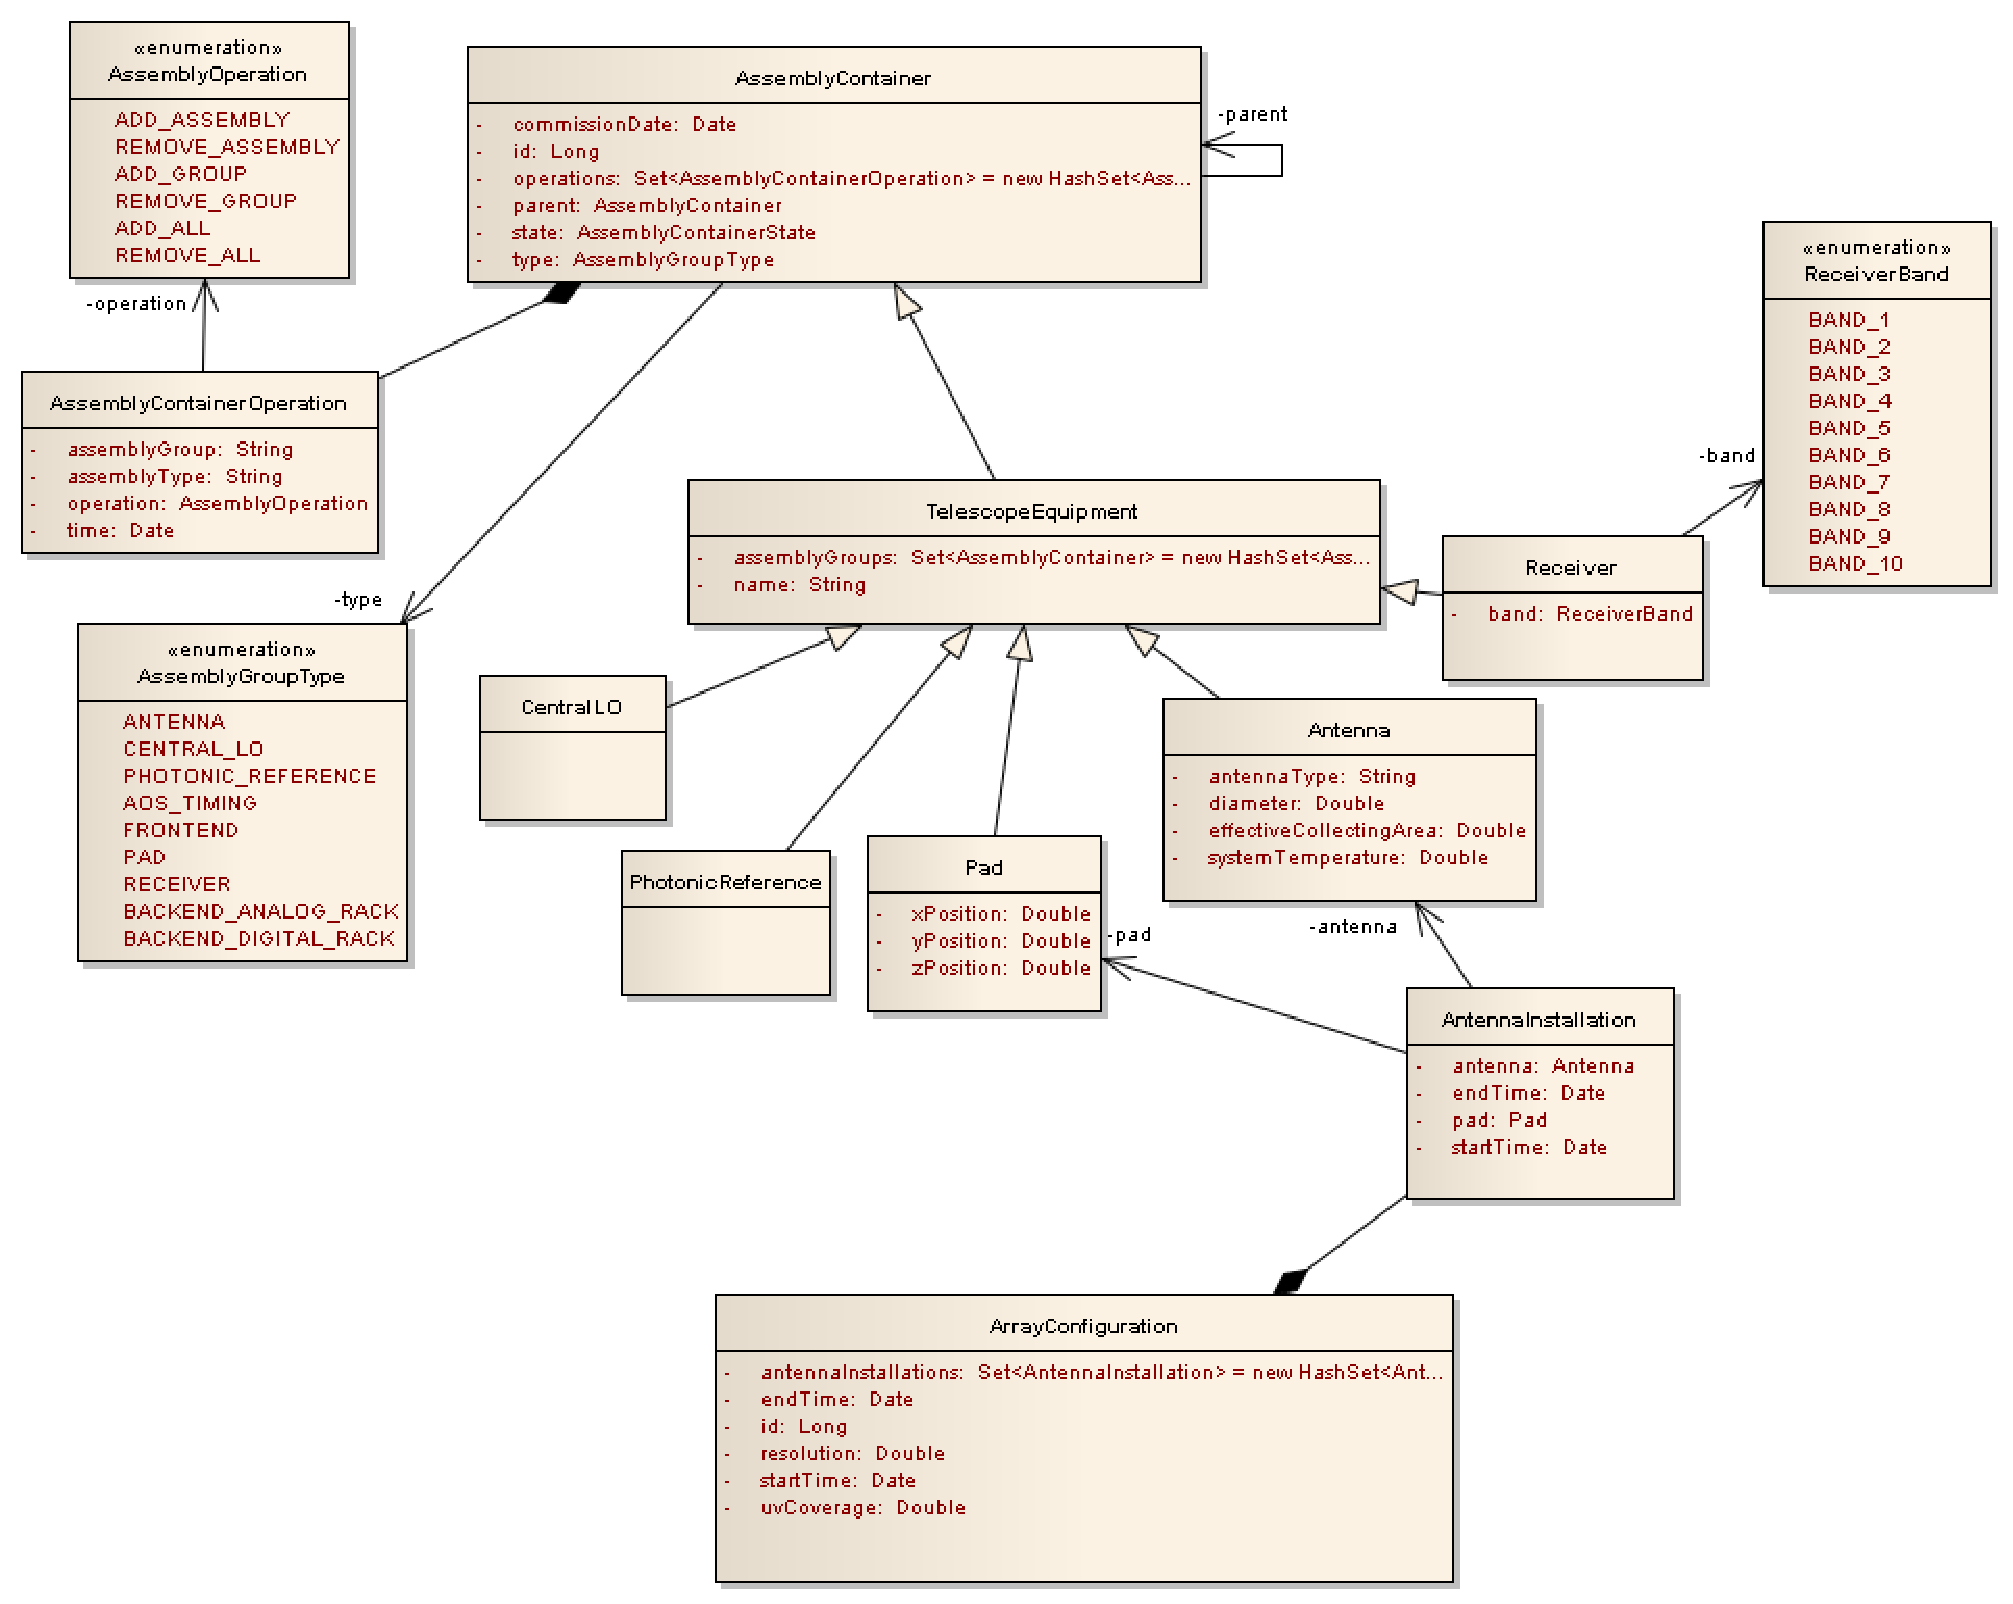
\includegraphics[width=0.67\textwidth]{images/Observatory}
\end{center}
\caption{Observatory instrumentation data model}
\label{fig:datamodel-observatory}
\end{figure}

The model designed for handle the Executive information and the observing season is represented in figure~\ref{fig:datamodel-executive}
The most relevant parts are: 
\begin{description}
\item[Executive] This class holds the information related to each executive provided as input. It saves the percentage and associates each Principal Investigator (class \textbf{PI}). Originally, the model was designed to allow to every PI have assigned percentages to each executive. However in practice, this has not been used.
\item[Observing Season] This class has the information relative to end and start dates for the observing season or observing cycle, also keeps the information relative to the daily schedule, in a \textbf{TimeInterval} instance.
\end{description}

\begin{figure}[htbp]	
\begin{center}
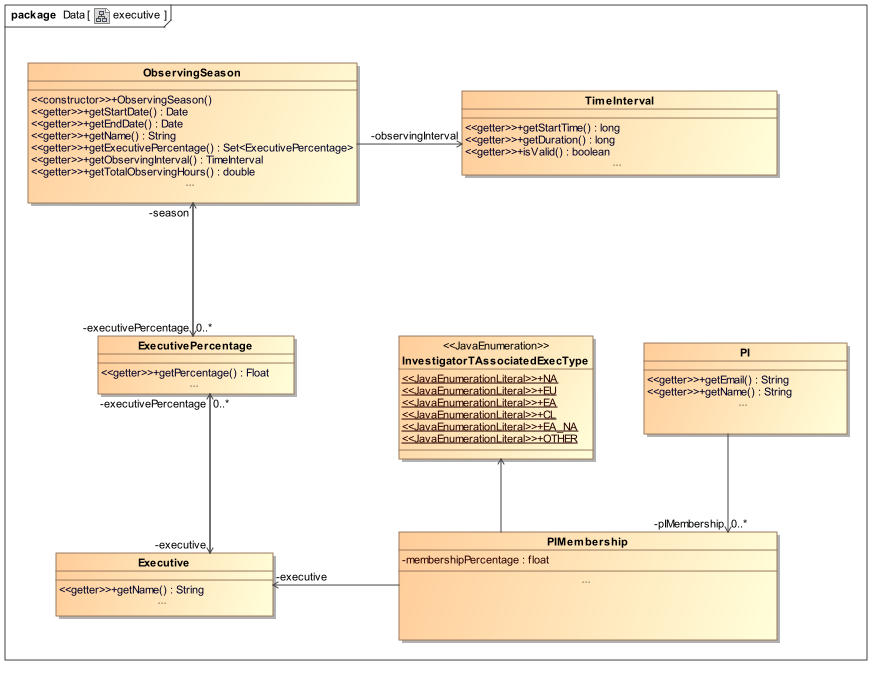
\includegraphics[width=0.67\textwidth]{images/Executive}
\end{center}
\caption{Executive and observing season data model}
\label{fig:datamodel-executive}
\end{figure}

The model designed for handle the weather is represented in figure~\ref{fig:datamodel-weather}. The weather model is quite simple, it has several classes holding data for the simulated weather, like precipitable water vapor, temperature, wind speed and phase. Also the model has the class \textbf{AtmParamters}, which contains the interpolation tables to calculate the atmospheric opacity.

\begin{figure}[htbp]	
\begin{center}
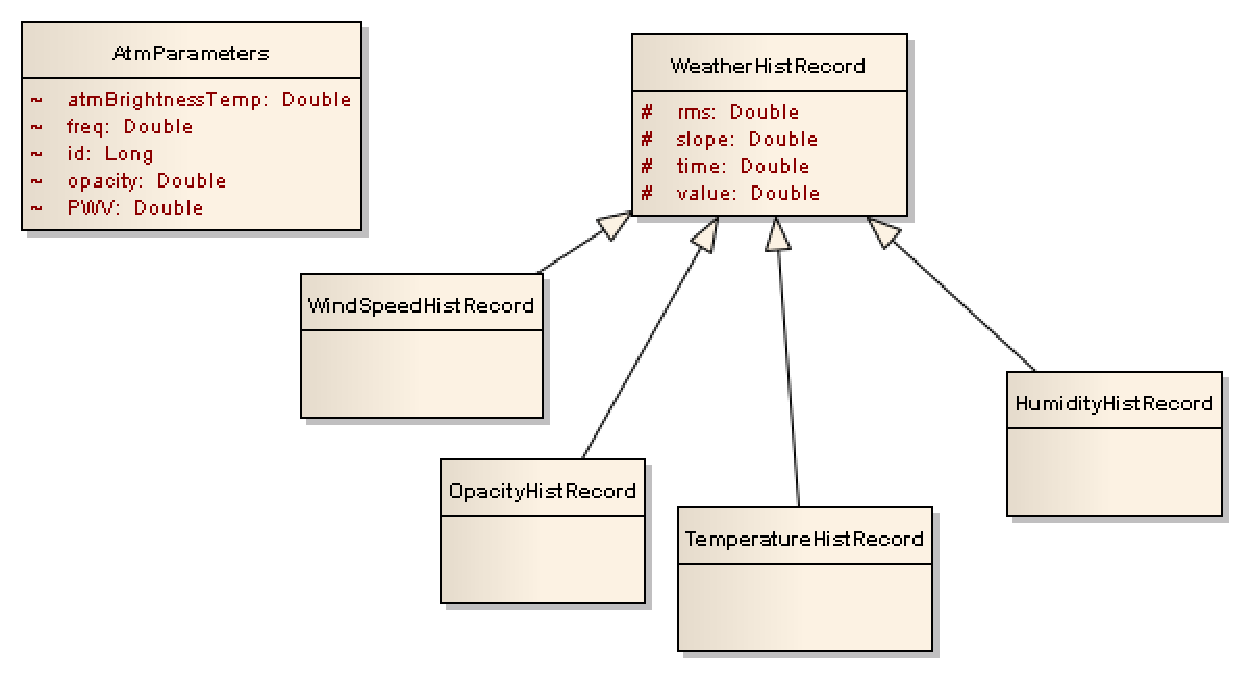
\includegraphics[width=0.67\textwidth]{images/Weather}
\end{center}
\caption{Weather data model}
\label{fig:datamodel-weather}
\end{figure}

The model designed for handle the observation progress status is represented in figure~\ref{fig:datamodel-observation}. This model defines \textbf{ExecBlock}, which keeps the time accounting and progress for each SB, array configuration and Executive. 

\begin{figure}[htbp]	
\begin{center}
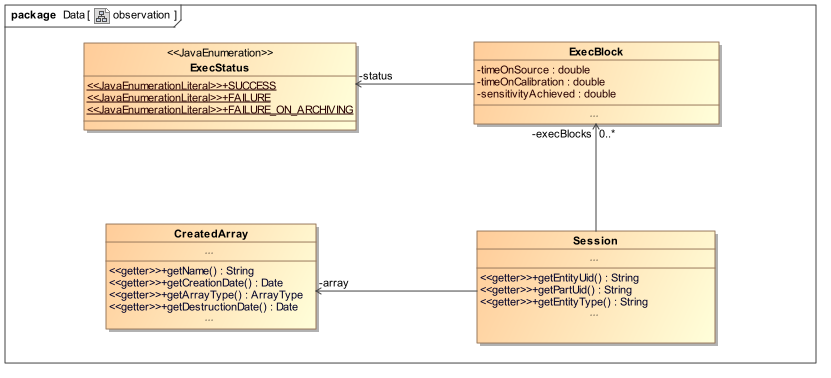
\includegraphics[width=0.67\textwidth]{images/Observation}
\end{center}
\caption{Observation progress status}
\label{fig:datamodel-observation}
\end{figure}

The top-level architecture of the ALMA's scheduling planning simulator is represented in diagram~\ref{fig:sim-top-level-architecture}. The software design uses as glue the Spring Core library, using Inversion of Control paradigm is possible to define via a configuration file, the objects to inject into the simulator, this includes Data Access Objects instances and the algorithm instances. It is enough for the software developed in this work to implement the correct interfaces to make them compatible with the rest of the ALMA software.

For the development of the validation software prepared for this work, some changes were done. Essentially the whole data source's code, presented in the left part and on bottom part of the figure~\ref{fig:sim-top-level-architecture}, which is particular to ALMA software, where replaced with a Data Accessors able to read the only the XML format defined by the scheduling subsystem software for data-interchange and with in-memory data structures part of the Java API, respectively. The core of the simulator tool and the algorithm does not deal directly with the data, instead a Data Accessors Object (DAO) interface was defined already by the ALMA's scheduling software, which abstracts all the interaction between the simulator and the data. Hence the replacement was fairly easy.

\begin{figure}[h!]	
\begin{center}
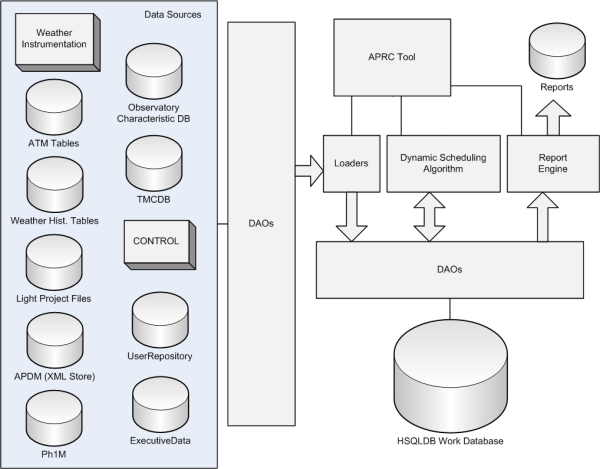
\includegraphics[width=0.67\textwidth]{images/simulator-arch}
\end{center}
\caption{Current top-level ALMA's scheduling simulator tool}
\label{fig:sim-top-level-architecture}
\end{figure}

In other hand, the algorithm implemented by ALMA software (DSA) was replaced with the modified Deficit Round-Robin algorithm implementation presented in this work (see chapter~\ref{sec:astro-schedule-problem}). The ALMA software design also make provisions at the algorithm level, defining an interface. Which, as well with the DAOs, was fairly easy to replace with new classes developed to implement the modified DRR algorithm.

\section {Simulation}
The simulator is the one used in the ALMA's scheduling subsystem. At the time when this document was written it remains mostly unchanged from its original design explained in detail in~\cite{hoffstadt10}. Nevertheless some modifications where done during the development of this work to support the simulation of several scenarios for the solution provided for the``Array configuration planning problem''. Next a briefly description of the simulator work-flow, shown in figure~\ref{fig:sim-state-machine}, is presented:

\begin{figure}[h!]	
\begin{center}
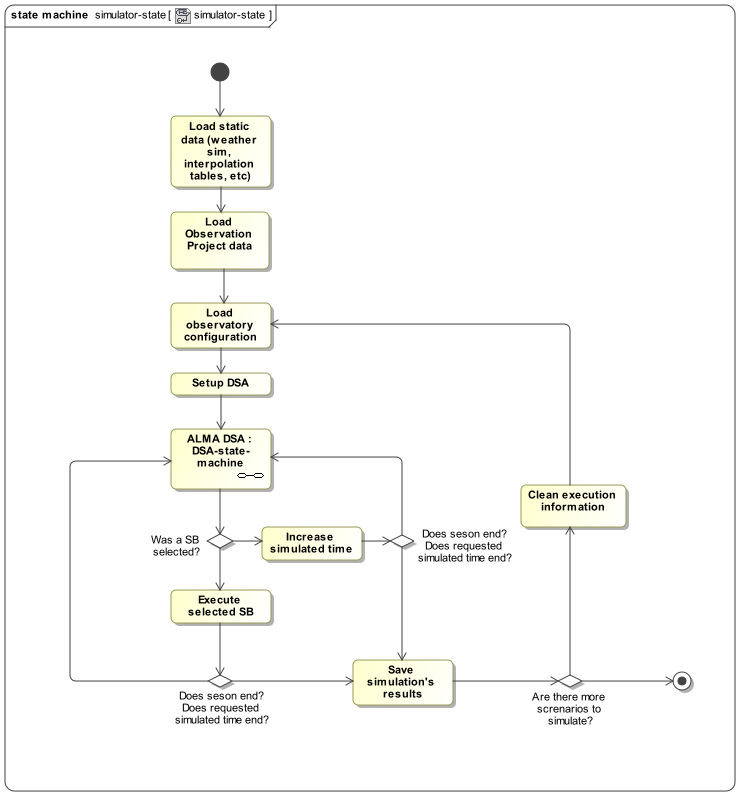
\includegraphics[width=0.67\textwidth]{images/simulator-state-machine}
\end{center}
\caption{ALMA simulator's state machine}
\label{fig:sim-state-machine}
\end{figure}

\begin{description}
\item[Load static data] \hfill \\
In this step the simulator will load all the immutable data from data-sources. This includes weather simulation data (temperature, humidity, wind speed, etc) and atmospheric interpolation tables to calculate the atmospheric opacity given the PWV and frequency. This step is separate from the rest of the date given that, the original ALMA's simulator is intended to be run using a relational database as back-end, then the data will be loaded just once.

During the development of this work, the simulator has been modified to work with data loaded completely in memory. Therefore this step add no value to the simulator itself. However it is worth of mention the difference with the original simulator used in ALMA software. 

\item[Load Observation project data] \hfill \\
In this step the simulator will load the data intended to be modified within the simulation procedure. This includes the whole observation projects, information relative to the executives and observing season.

\item[Load observatory configuration] \hfill \\
In this step the simulator loads or modifies the array configuration planning for the observing season. Originally the ALMA's simulator supported only the loading of this data from the data-sources. During the development of this work this step was separated from the previous one, to support the setup of multiple scenarios for the, already configured, observing season.

\item[Setup DSA (algorithm for Astronomical observation scheduling problem)] \hfill \\
In this step the different simulations for each array configuration are scheduled. The simulator, according to its progress, will change among the different array configurations prepared in this step. If the simulator detects that there are no more configurations remaining for the rest of the simulated duration, then it will terminate the simulation execution and it will prepare the results and output them.

\item[Running DSA (DSA-state-machine)] \hfill \\
In this step the DSA will execute according to the work-flow presented in figure~\ref{fig:sched-dsa-state-machine} and explained in section~\ref{sec:astro-schedule-problem}.

If the DSA returns no result, then the simulator will jump $1\,[h]$ and $20\,[m]$ its simulation and try again checking whether there are selectable scheduling blocks or not. The simulator will do this until the array end time is reached.

\item[Save simulation's result] \hfill \\
After every simulation is complete, then the simulator will dump an XML file containing most of the information for post-analysis.

\item[Clean execution information] \hfill \\
Since during simulation certain data for the Scheduling blocks are filled (like current number of repetitions and total time duration) and executive accounting is modified. It is necessary to clean-up all the modified data. 

The implementation done for this work will clean the complete context used for simulation, and it will reload all the data from scratch. Although it is known that this produce an overhead for the testing, it is safer to reload all the date to avoid to find programming defects during testing.

\end{description}

\section {Input Data}
\label{sec:input-data}
This section summarizes the data that will be used to validate the solutions. 

\subsection{Observing Season and executives time share}
The executive time share configuration is presented in table~\ref{table:input-executive}

\begin{table}[h!]
\begin{center}
\begin{tabular}{|c|c|}
\hline
Executive & Time (\%)\\ \hline
CL & $9.5\%$ \\ \hline
EA & $21.375\%$ \\ \hline
EA\_NA & $0.0\%$\tablefootnote{For accounting purposes, the used time is split in equal parts between EA \& NA} \\ \hline
EU & $32.0625\%$ \\ \hline
NA & $32.0625\%$ \\ \hline
OTHER & $5.0\%$ \\ \hline
\end{tabular}
\end{center}
\caption{Time share partition given to each Executive}
\label{table:input-executive}
\end{table}

The following are the details for the observation season:

\begin{description}
\item[Start date]: June 1st, 2014 00:00 UTC 
\item[End date]: October 1st, 2015 00:00 UTC
\item[Start hour daily observation interval]: 23:00 UTC
\item[End date daily observation interval]: 09:00 UTC
\item[Total number of hours available for science]: $4861\,[h]$
\end{description}

\subsection{Array Configurations}

One specific requirement for the algorithms presented in this work, is that the configurations must be available as part of the input. These configurations were already discussed by groups internal to the observatory, whom determines what are the capabilities offered to the science community before the announcement of a new observation season.

\begin{table}[h!]
\begin{center}
\begin{tabular}{|c|c|c|c|}
\hline
Configuration name & Array type & Min. Baseline $[m]$ & Max. Baseline $[m]$\\
\hline
C34-1 & $12\,[m]$ & $14.2$ & $165.6$ \\
\hline
C34-2 & $12\,[m]$ & $14.1$ & $303.6$ \\
\hline
C34-3 & $12\,[m]$ & $20.6$ & $442.7$ \\
\hline
C34-4 & $12\,[m]$ & $20.6$ & $558.2$ \\
\hline
C34-5 & $12\,[m]$ & $25.8$ & $820.2$ \\
\hline
C34-6 & $12\,[m]$ & $40.6$ & $1091.0$ \\
\hline
C34-7 & $12\,[m]$ & $40.6$ & $1507.9$ \\
\hline
7m    & $7\,[m]$  & $8.9$  & $32.1$ \\
\hline
TP    & $TP$      & $-$    & $-$ \\
\hline
\end{tabular}
\end{center}
\caption{Array configurations provided as input for the algorithms}
\label{table:input-array-configs}
\end{table}

For ALMA' s cycle 2, the list of the array configurations is presented in table~\ref{table:input-array-configs}. Although the table does not introduce the starting and ending dates for any of the configurations, which are part of the problems presented in this work, and solved by the algorithms introduced in this document.


\subsection{Observation projects}
As input for the validation tests and benchmarking of the software developed in this work, there will be used the cycle 2 proposals submitted to ALMA observatory, although these proposals have been already processed and converted into APDM Observation projects and APDM Scheduling Blocks, the data used for tests is an extract of them, this data contains only the relevant parts for the scheduling simulation.

At the moment of write this document, the Observation Projects are not still publicly available, but according to ALMA observatory policy, they will become available at the end of 2014 or beginning of 2015. 

A summary of the Scheduling blocks that the validation will be used is presented in table~\ref{table:requested-time-12m} for $12\,[m]$ array configurations, in table~\ref{table:requested-time-7m} for $7\,[m]$ array configurations and in table~\ref{table:requested-time-tp} for $TP$  array configurations. Each table have in detail the number of hours requested for each executive, broke down the time per science grade. $D$ graded projects are not shown in the tables, although they are available as part of the data set used as input.

\begin{table}
\begin{center}
\begin{tabular}{|c|c|c|c|}
\hline
Grade & Executive & Time Requested $[h]$ & Number of Scheduling Blocks \\ \hline
A &	CL		& 12.0  & 2 \\ \hline
A &	EA		& 36.0  & 13 \\ \hline
A &	EA/NA	& 6.0   & 3 \\ \hline
A & EU      & 112.0 & 31 \\ \hline 
A &	NA		& 114.0	& 31 \\ \hline
A & OTHER	& 0		& 0 \\ \hline
B  & CL 	& 160.0		& 48  \\ \hline
B  & EA     & 438.0     & 145 \\ \hline
B  & EA/NA  & 106.0     & 30  \\ \hline
B  & EU     & 828.0     & 280 \\ \hline
B  & NA     & 1024.0    & 344 \\ \hline
B  & OTHER  & 40.0      & 19  \\ \hline
C  & CL     & 130.0     & 50  \\ \hline
C  & EA     & 246.0     & 65  \\ \hline
C  & EA/NA  & 52.0      & 23  \\ \hline
C  & EU     & 410.0     & 155 \\ \hline
C  & NA     & 556.0     & 196 \\ \hline
C  & OTHER  & 34.0      & 13  \\ \hline
\end{tabular}
\end{center}
\caption{Requested time for $12m$ array configurations}
\label{table:requested-time-12m}
\end{table}

\begin{table}
\begin{center}
\begin{tabular}{|c|c|c|c|}
\hline
Grade & Executive & Time Requested $[h]$ & Number of Scheduling Blocks \\ \hline
A &	CL		& 0  & 0 \\ \hline
A &	EA		& 24.0  & 1 \\ \hline
A &	EA/NA	& 6.0   & 12 \\ \hline
A & EU      & 12.0 & 1 \\ \hline 
A &	NA		& 16.0 & 2 \\ \hline
A & OTHER	& 0		& 0 \\ \hline
B  & CL 	& 16.0		& 1  \\ \hline
B  & EA     & 78.0     & 21 \\ \hline
B  & EA/NA  & 22.0     & 5  \\ \hline
B  & EU     & 168.0     & 41 \\ \hline
B  & NA     & 182.0    & 29 \\ \hline
B  & OTHER  & 0.0      & 0  \\ \hline
C  & CL     & 38.0     & 2  \\ \hline
C  & EA     & 46.0     & 12  \\ \hline
C  & EA/NA  & 36.0      & 9  \\ \hline
C  & EU     & 5800     & 7 \\ \hline
C  & NA     & 556.0     & 196 \\ \hline
C  & OTHER  & 72.0      & 12  \\ \hline
\end{tabular}
\end{center}
\caption{Requested time for $7m$ array configurations}
\label{table:requested-time-7m}
\end{table}

\begin{table}
\begin{center}
\begin{tabular}{|c|c|c|c|}
\hline
Grade & Executive & Time Requested $[h]$ & Number of Scheduling Blocks \\ \hline
A &	CL		& 0  & 0 \\ \hline
A &	EA		& 28.0  & 1 \\ \hline
A &	EA/NA	& 208.0   & 2 \\ \hline
A & EU      & 132.0 & 1 \\ \hline 
A &	NA		& 112.0 & 2 \\ \hline
A & OTHER	& 0		& 0 \\ \hline
B  & CL 	& 28.0		& 1  \\ \hline
B  & EA     & 1852.0     & 21 \\ \hline
B  & EA/NA  & 752.0     & 5  \\ \hline
B  & EU     & 922.0     & 41 \\ \hline
B  & NA     & 1792.0    & 29 \\ \hline
B  & OTHER  & 0.0      & 0  \\ \hline
C  & CL     & 52.0     & 2  \\ \hline
C  & EA     & 1250.0     & 12  \\ \hline
C  & EA/NA  & 824.0      & 9  \\ \hline
C  & EU     & 368.0     & 7 \\ \hline
C  & NA     & 78.0     & 12 \\ \hline
C  & OTHER  & 2.0      & 1  \\ \hline
\end{tabular}
\end{center}
\caption{Requested time for $TP$ array configurations}
\label{table:requested-time-tp}
\end{table}

